% !TEX root = ./cvl.tex

\section{Implementation}
\label{sec:implementation}

In this section, we present how our implementation makes use of in-database execution to provide scalability and engine reuse for CVL (Section~\ref{sec:implementation:indatabase}). In addition, we discuss a number of extensions to CVL that we found to be useful for practical applications (Section~\ref{sec:implementation:extensions}). 

\subsection{In-Database Execution}
\label{sec:implementation:indatabase}

\minisec{Overview}
Since CVL is declarative, and CVL constraints are already expressed in SQL, it is natural to attempt to reuse as much existing DBMS technology as possible to execute CVL. Figure~\ref{fig:indatabase} shows how CVL is compiled for execution in a relational DBMS, which acts as the language runtime. The output of the CVL compiler is a database script for the target host, containing both SQL and stored procedures, and following the algorithmic framework of Figure~\ref{fig:algorithmic-framework}. The script is pushed down to the database engine, and operates against the appropriate input data stored in the system. This strategy offers us two main advantages:

\begin{enumerate}

\item Since all code is pushed down and both input and output reside in the database, we do not need to transfer any data outside of the database engine. This co-location of code and data is a significant advantage for large datasets.

\item By expressing as much as possible of the generated code in SQL, we can reuse decades of optimizations built into database engines, especially for geospatial data~\cite{Guttman1984:RTree,Hellerstein1995:GiST}. This opens up many opportunities, such as automatic optimization, parallelism, and selection of specialized algorithms and indexes.  

\end{enumerate} 

While the general strategy of compiling declarative languages to SQL has been pursued in other contexts, e.g., for XQuery~\cite{pathfinder} and LINQ~\cite{ferry}, our context poses a particular challenge of integrating the language with algorithmic solvers inside the database. 

\begin{figure}[htbp]
\begin{center}
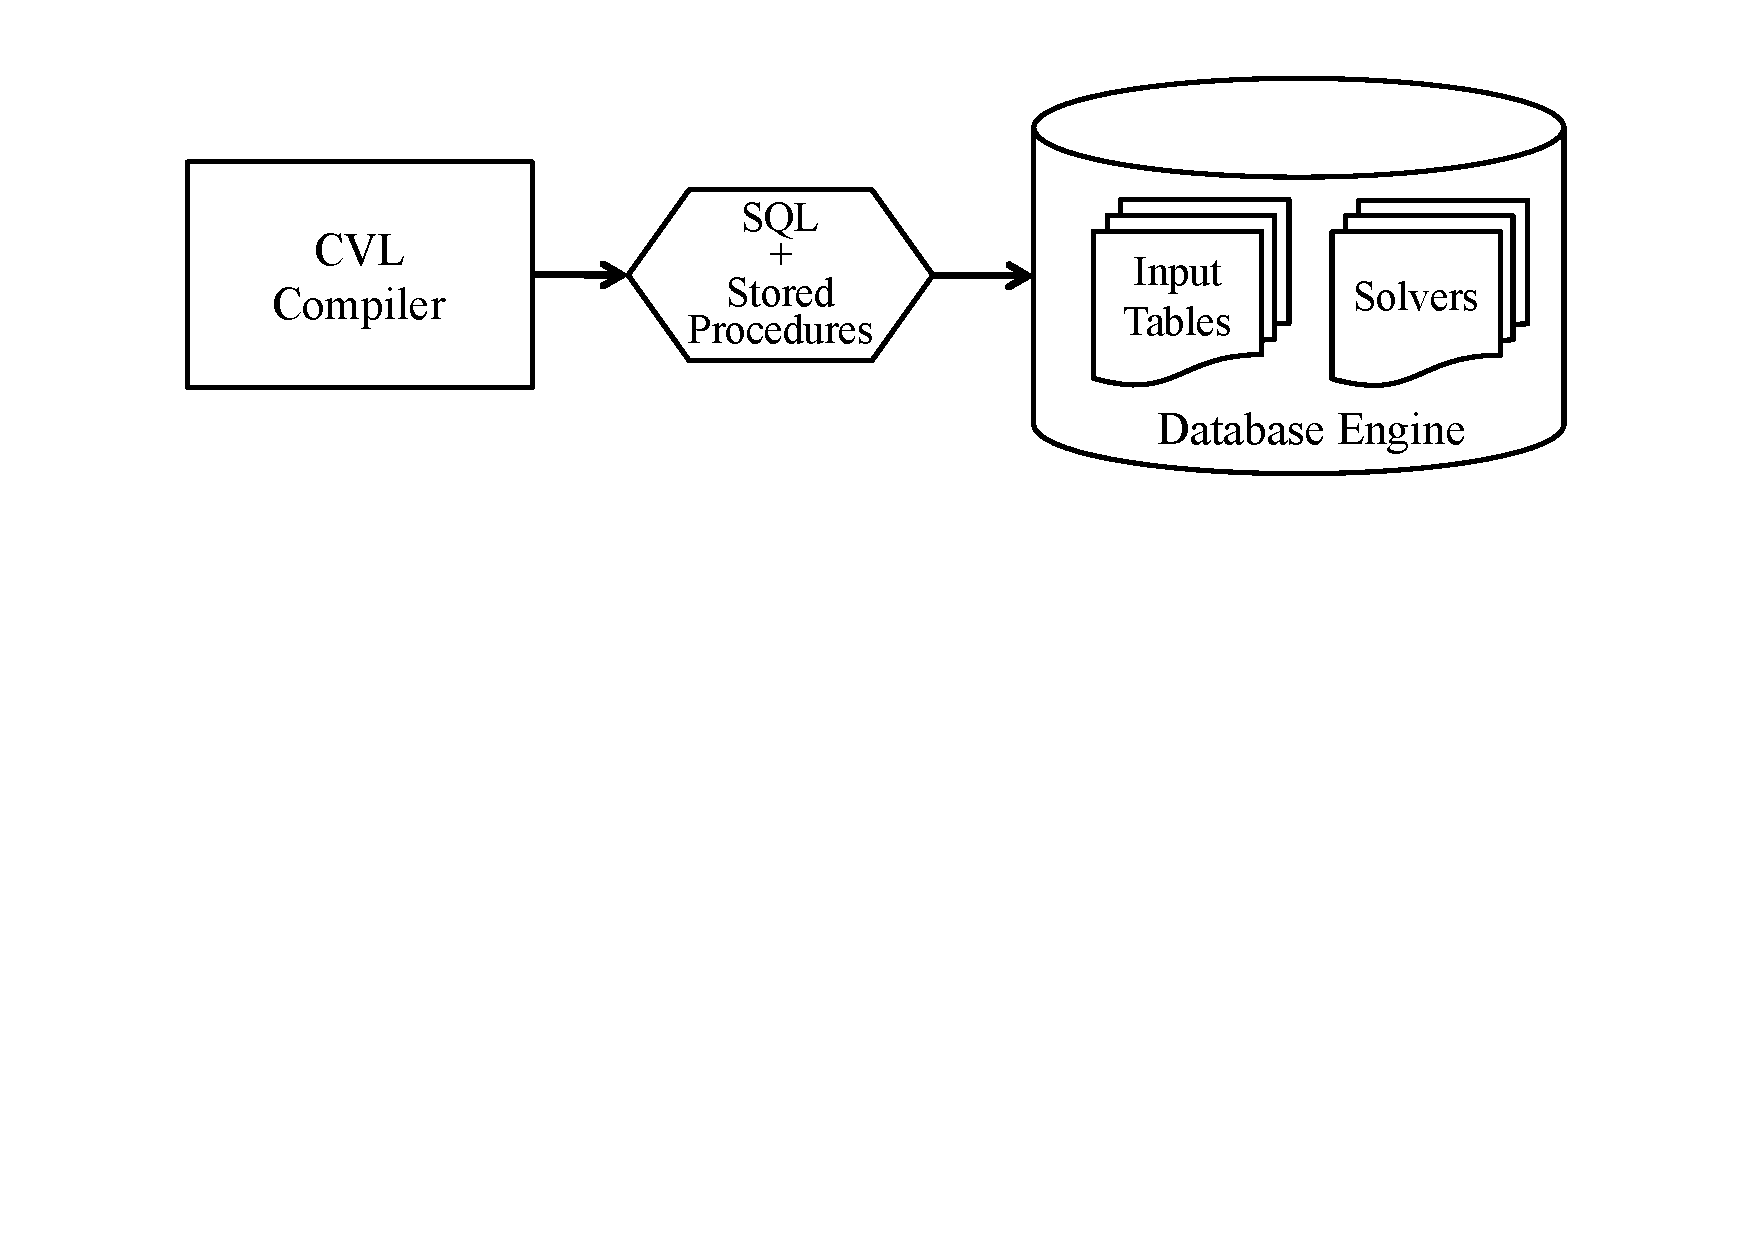
\includegraphics[scale=.35,viewport=400 375 450 550]{figs/indatabase-execution.pdf}
\caption{CVL and in-database execution.}
\label{fig:indatabase}
\end{center}
\end{figure}

\minisec{Solvers}
In Section~\ref{sec:algorithms}, we have presented two different algorithmic approaches for solving CVL generalizations: static greedy (SGA), LP-based greedy (LPGA). We now show how to express each of these approaches in SQL along with stored procedures. 

SGA is the simplest algorithm, and recall that it operates independently on the conflicts generated by each constraint. Suppose the conflicts $C$ generated by the active constraints are stored in a \emph{conflicts} table. Then for constraint $c \in C$, SGA is tantamount to the query:

\begin{lstlisting}
SELECT rid
FROM (
  SELECT ROW_NUMBER() 
         OVER (PARTITION BY cid
               ORDER BY cvl_rank) AS r,
         rid, cvl_rank, lambda_c
  FROM conflicts) h
WHERE h.r <= h.lambda_c
\end{lstlisting}

For each conflict set $c$, we order records by rank, and ensure that we pick at least $\lambda_c$ records. The declarative formulation allows us to reuse optimized sorting code in the database engine for execution.

LPGA solves a linear programming relaxation of the set multicover problem. We express LPGA by a stored procedure. The procedure accesses the conflicts for the constraints via SQL, constructs an appropriate LP, and then calls into an LP solver library~\cite{cvxopt}. Since the solver library does not use built-in database optimizations, this execution strategy for LPGA only leverages the first advantage of data and code co-location listed above.

Finally, note that the code for finding conflict sets is already expressed in SQL by the user for each constraint. As a consequence, this user code can make use of all built-in database optimizations available in the target engine.

\minisec{CVL runtime functions}
In the definition of the visibility constraint in Section~\ref{sec:create:constraint:statement} we reference two stored procedures in the CVL runtime library, \texttt{CVL\_PointHash} and \texttt{CVL\_WebMercatorCells}. These functions are implemented in SQL and make use of the spatial extension of the database~\cite{postgis}.

The procedure \texttt{CVL\_PointHash} uses a call to \texttt{ST\_GeoHash} to implement an injective mapping from points to strings. These strings are used as unique $cid$s for the visibility constraint.  

The \texttt{CVL\_WebMercatorCells} function maps a geometry at a given zoom-level to centroids of all intersected tiles (on that zoom-level). We experimented with several ways to do this for general geometries (points, line segments, polygons) and found that rasterizing the geometry (using the function \texttt{ST\_AsRaster} in the spatial extension of the database) and iterating over the indices was the fastest for general geometries. For point records it is significantly faster to use the standard transformation function \texttt{ST\_SnapToGrid}.

An improvement to \texttt{CVL\_WebMercatorCells} that we did not have time to implement is to compute tiles as quad-keys on the highest level only. Tile identifiers for lower levels are easily computed by taking prefixes of the quad-keys. This approach only benefits the running time when using constraints that are tile-based.

\subsection{Extensions}
\label{sec:implementation:extensions}

When designing CVL, we discussed a number of our decisions with geospatial map developers at GST. These discussions, along with our implementation experience of CVL use cases, led us to a set of extensions over the core language targeted at improving convenience of use. We present these extensions below.

\marcos{Either introduce GST in Intro or remove reference above.}

\minisec{Partitioning and Merging Datasets} 
A single input table may contain geospatial objects of different classes, e.g., roads and points of interest. When this is the case, users often wish to generalize some of these classes of objects independently, but obtain a single result map. While this can be done by merging the results of multiple GENERALIZE statements, we found it useful to add syntactic sugar to support this case. We extend the GENERALIZE statement with PARTITION BY and MERGE PARTITIONS clauses. PARTITION BY allows us to effectively segregate the input into multiple independent sets. MERGE PARTITIONS combines a few of these sets before providing them as input to generalization. For example, assume a \emph{geo\_objects} table contains highways, roads, restaurants, and hotels, tagged by a \emph{type} attribute. We could then generalize \emph{geo\_objects} as follows:

\begin{lstlisting}
GENERALIZE  geo_objects
TO network_and_poi_map
...
PARTITION BY type
MERGE PARTITIONS 'restaurant', 'hotel' 
              AS 'poi'
... 
\end{lstlisting}

In the example, we overlay independent generalizations of highways, roads, and points of interest into a single map. However, restaurants and hotels are generalized as a single input set.  

\minisec{Forced and All-or-Nothing Visualization}
Intuitively, constraints let users specify what is \emph{not} allowed in a given map, by forbidding the existence of conflicts. However, users also find helpful to control certain behaviors that \emph{must} occur in their map. We extended the GENERALIZE statement with support for two types of behaviors: (1)~the ability to mandate a minimum zoom level for a particular partition of the input, and (2)~the ability to force that either all or none of the objects of a given partition be displayed. For example, a user may wish to specify that highways must only appear at zoom level 10 or lower in their map. In addition, for consistency, either the whole highway skeleton is displayed or no highways should show up. To achieve this goal, we extend the GENERALIZE statement by a FORCE clause with MIN LEVEL and ALLORNOTHING specifiers. Continuing the example above:

\begin{lstlisting}
...
FORCE MIN LEVEL 10 ALLORNOTHING FOR 'highway'
... 
\end{lstlisting}

In the evaluation of CVL, the minimum level specifier controls what data is given as input for a zoom level. The all-or-nothing specifier, on the other hand, controls filtering of the output of the level generalization process. If the specifier is present, all records of a partition are eliminated if any record from the partition input is not present in the output. By filtering output, we ensure that the result also respects all other constraints specified by the user. 

%\minisec{Set up and Tear Down for Constraints}   
%Map constraints can exhibit significant complexity. Since a constraint is expressed as a single SELECT statement, it is often helpful to be able to refer to temporary tables in its formulation. We have thus extended the CREATE CONSTRAINT statement to include two additional clauses: WITH SETUP and WITH TEARDOWN. The former allows a user-defined SQL statement to be executed in advance of the constraint evaluation, creating any supporting tables for the evaluation of the constraint. The latter specifies user-defined cleanup code. Note that since constraints are evaluated independently at each zoom level, the set-up and tear-down clauses are evaluated before and after the constraint SQL at each zoom level.       
%\marcos{Move necessary information from paragraph above to Language section, and remove paragraph after that.}

%
% MVS: We can probably get away with not showing the syntax below. 
%
%\begin{lstlisting}
%CREATE CONSTRAINT C1 
%AS NOT EXISTS
% (SELECT cid, rid, minhits
%  FROM {more SQL})
%WITH SETUP
% {user-defined SQL}
%WITH CLEANUP
% {user-defined SQL}
%\end{lstlisting}

